\documentclass[11pt]{article}
%%%%%%%%%%%%%%%%%%%%%%%%%%%%%%%%%%%%%%%%%%%%%%%%%%%%%%%%%%%%%%%%%%%%%%%%%%%%%%%%%%%%%%%%%%%%%%%%%%%%%%%%%%%%%%%%%%%%%%%%%%%%%%%%%%%%%%%%%%%%%%%%%%%%%%%%%%%%%%%%%%%%%%%%%%%%%%%%%%%%%%%%%%%%%%%%%%%%%%%%%%%%%%%%%%%%%%%%%%%%%%%%%%%%%%%%%%%%%%%%%%%%%%%%%%%%
\usepackage{amsmath}
\usepackage{amssymb}
\usepackage{amsfonts,color}
\usepackage{mathtools}
\mathtoolsset{showonlyrefs}

\usepackage{natbib}

\usepackage[normalem]{ulem}
\usepackage{caption}
\usepackage{subcaption}

\setlength{\textwidth}{16cm}
\setlength{\textheight}{24cm}
\topmargin=-2cm
\setlength{\hoffset}{-1.4cm}
\begin{document}


\qquad

\qquad

\qquad


\qquad

\qquad

\qquad

\newcommand{\thedate}{\today}

\thedate

\qquad

\qquad

\qquad



Dear Editor,

\qquad


We would be very grateful if you would consider this revision, entitled \emph{`On the estimation of the number of components in multivariate functional principal component analysis'} for publication in \emph{Communications in Statistics - Simulation and Computation}. We were able to address the comments made by the reviewers and to strengthen our results. A point-to-point reply is provided below. 

\quad

We quite naturally hope that this version matches reviewers' expectations, and we thank you in advance for your consideration.



\quad


Sincerely, 

\medskip



 Steven Golovkine 
 \\(on behalf of the co-authors  Edward Gunning, Andrew J. Simpkin and Norma Bargary)





\newpage


\begin{center}
{\large Comments received for \emph{On the estimation of the number of components in multivariate functional principal component analysis}}\\
\end{center} 


The changes are in \textcolor{blue}{blue} in the main text.
\vspace*{1cm}


{\large \textbf{Reviewer 1} }


\bigskip

\itshape


\textbf{Comment \#1 :}

Although I understand how $s_1, \dots , s_p$ are obtained, the authors need to provide a more detailed explanation of how these values are generated using a Bernoulli distribution, for example.

\medskip

\normalfont

\textbf{Reply:} The sentence ``generated according to a Bernoulli distribution'' has been added to the text.


\bigskip

\itshape

\textbf{Comment \#2 :}

It would be helpful to simulate a case with irregular time points, where each function has different time points. Moreover, the time points for each function do not need to be regular. I recommend that the authors consider these situations.

\medskip

\normalfont

\textbf{Reply:}


\bigskip

\itshape


\textbf{Comment \#3 :}

The paragraph in the end of Page 2 and Page 3 requires a complete rewrite as it lacks the necessary rigor in its explanations and methodology.

\medskip

\normalfont

\textbf{Reply:}



\bigskip


\itshape


\textbf{Comment \#4 :}

The simulation study and application sections of the paper need to be significantly revised. The current writing provides very limited explanation, which makes it difficult for readers to fully understand the intuition behind the results, the significance of the findings, and how the method performs in practice. The authors should offer more detailed descriptions of the simulation settings including the rationale behind the chosen parameters and models. Moreover, the application section should clearly describe the dataset, the variables used, and how the results from the method apply to real-world scenarios. More emphasis should be placed on interpreting the application results and their implications which help readers understand the practical value of the proposed method.


\medskip

\normalfont

\textbf{Reply:}



\bigskip

\itshape



\textbf{Comment \#5 :}

The authors classify the number of simulations based on the size of the circles, which is very confusing. Please present the results using a clearer visualization method.

\medskip

\normalfont

\textbf{Reply:} We replace the plot by different tables presenting the results.


\bigskip


\itshape

\textbf{Comment \#6 :}

The authors use B-spline bases for the Canadian weather dataset. I recommend that they also use a Fourier basis and compare the results. This can demonstrate the robustness of the method, as Fourier bases typically provide a better fit for weather data.


\medskip

\normalfont

\textbf{Reply:} We recall that our aim is to ``provide commentary on the estimation of the number of principal components utilising the methodology devised in \cite{happMultivariateFunctionalPrincipal2018}''. We provide, here, the estimated eigenfunctions after smoothing the data using $10$ Fourier. The results are the same than with the B-splines basis. 

\begin{figure}[!h]
     \centering
     \begin{subfigure}[b]{0.49\textwidth}
         \centering
         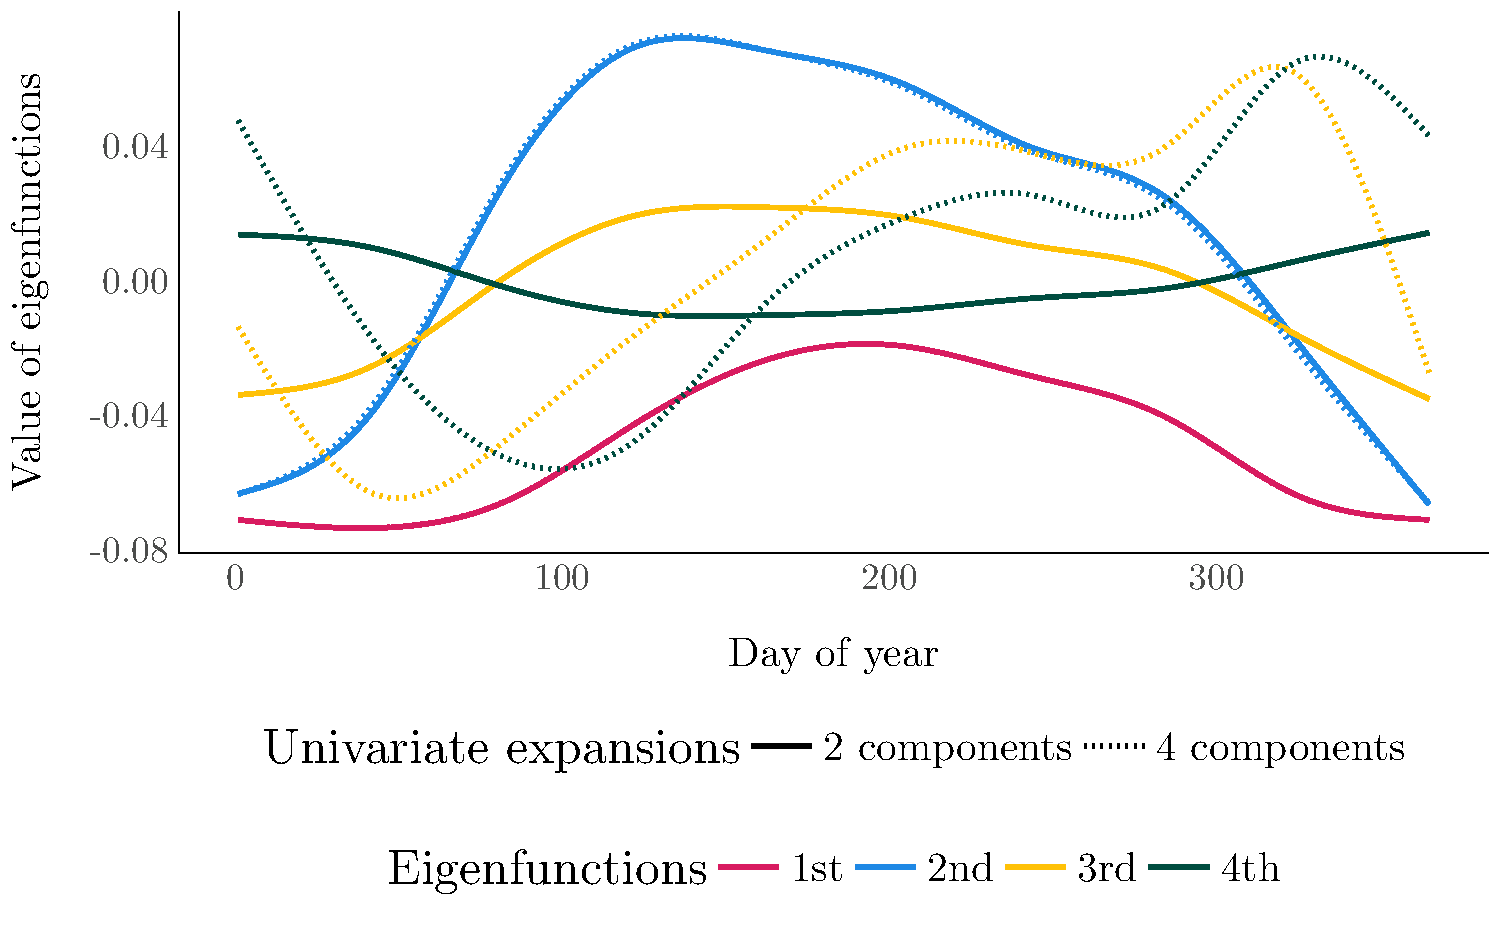
\includegraphics[width=1\textwidth]{temperature_eigen_fourier.pdf}
         \caption{Temperature (first component)}
         \label{fig:temperature}
     \end{subfigure}
     \hfill
     \begin{subfigure}[b]{0.49\textwidth}
         \centering
         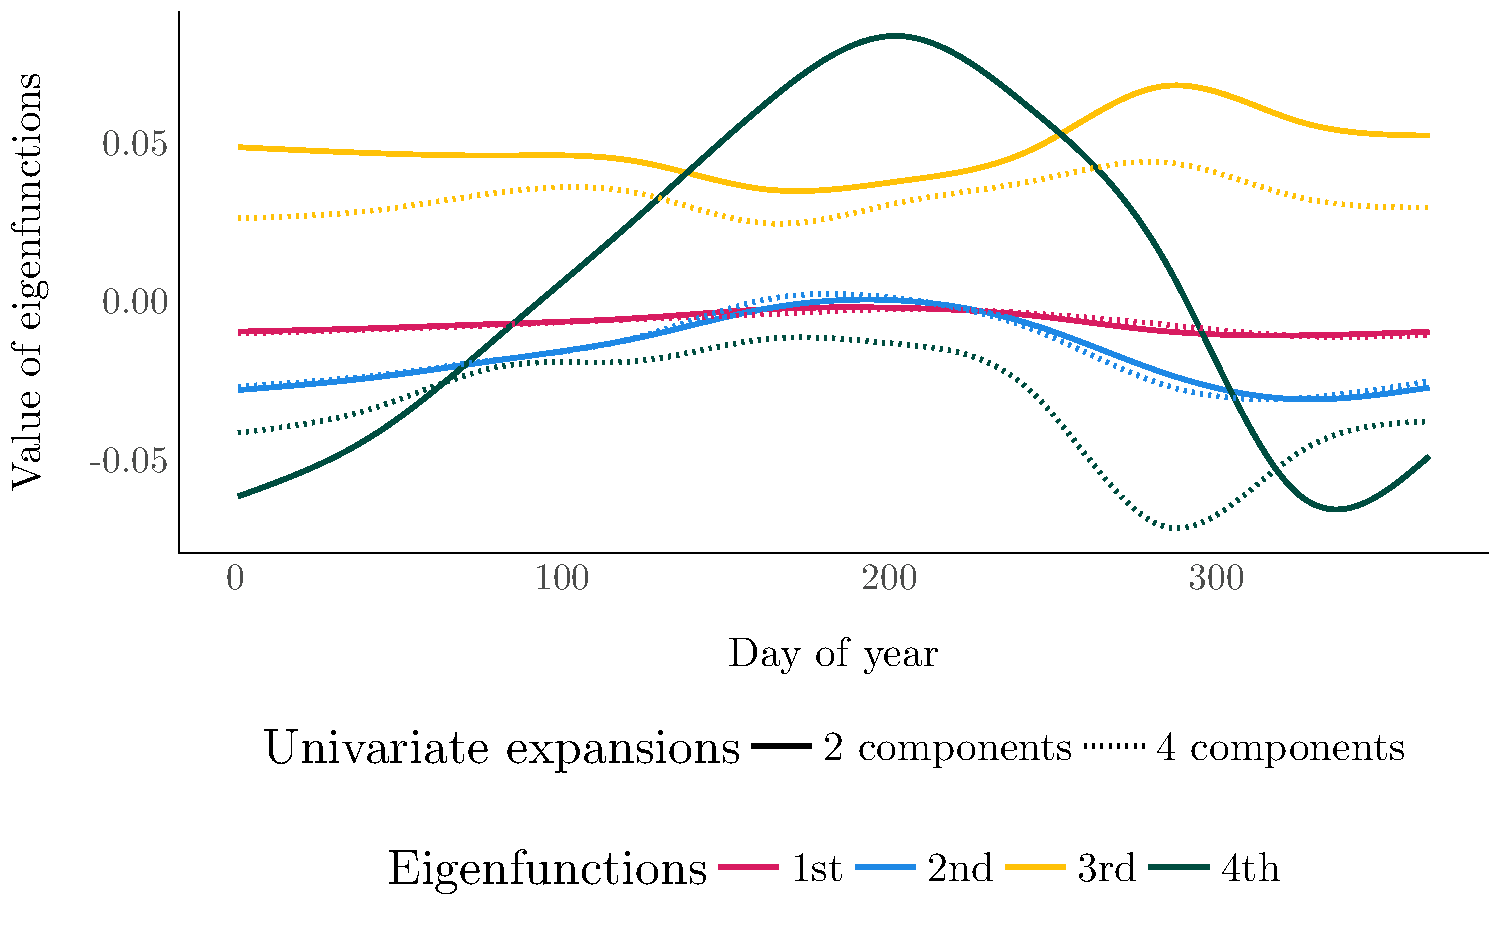
\includegraphics[width=1\textwidth]{precipitation_eigen_fourier.pdf}
         \caption{Precipitation (second component)}
         \label{fig:precipitation}
     \end{subfigure}
     \caption{Estimation of the first four eigenfunctions of the Canadian weather dataset using using two and four univariate components for the univariate expansions after Fourier basis smoothing.}
     \label{fig:eigenfunctions_weather}
\end{figure}


\bigskip


\itshape

\itshape

\textbf{Comment \#7 :}

Figure 3 is missing a y-axis.

\medskip

\normalfont

\textbf{Reply:} We added y-axis to Figure 3.



\bigskip




{\large \textbf{Reviewer 2} }


\bigskip

\itshape


\textbf{Comment \#1 :}

The manuscript needs English proofreading.

\medskip

\normalfont

\textbf{Reply:} 

Three of the four authors are English native speakers. 

\bigskip

\itshape

\textbf{Comment \#2 :}

What is the limitation of the proposed approach?

\medskip

\normalfont

\textbf{Reply:} 

We recall that our aim is to ``provide commentary on the estimation of the number of principal components utilising the methodology devised in \cite{happMultivariateFunctionalPrincipal2018}''. We are not proposing a new approach but comment on the limitation of the approach proposed in \cite{happMultivariateFunctionalPrincipal2018}.

\bigskip


\bibliographystyle{plainnat}
\bibliography{biblio} 

\end{document} 